\documentclass[landscape,final,a0paper,fontscale=0.285]{baposter}

\usepackage{calc}
\usepackage{graphicx}
\usepackage{amsmath}
\usepackage{amssymb}
\usepackage{relsize}
\usepackage{multirow}
\usepackage{rotating}
\usepackage{bm}
\usepackage{url}

\usepackage{graphicx}
\usepackage{multicol}

%\usepackage{times}
%\usepackage{helvet}
%\usepackage{bookman}
\usepackage{palatino}

\newcommand{\captionfont}{\footnotesize}

\graphicspath{{images/}{../images/}}
\usetikzlibrary{calc}

\newcommand{\SET}[1]  {\ensuremath{\mathcal{#1}}}
\newcommand{\MAT}[1]  {\ensuremath{\boldsymbol{#1}}}
\newcommand{\VEC}[1]  {\ensuremath{\boldsymbol{#1}}}
\newcommand{\Video}{\SET{V}}
\newcommand{\video}{\VEC{f}}
\newcommand{\track}{x}
\newcommand{\Track}{\SET T}
\newcommand{\LMs}{\SET L}
\newcommand{\lm}{l}
\newcommand{\PosE}{\SET P}
\newcommand{\posE}{\VEC p}
\newcommand{\negE}{\VEC n}
\newcommand{\NegE}{\SET N}
\newcommand{\Occluded}{\SET O}
\newcommand{\occluded}{o}
\newcommand{\toolname}{\textsc{Visualizer} }
%%%%%%%%%%%%%%%%%%%%%%%%%%%%%%%%%%%%%%%%%%%%%%%%%%%%%%%%%%%%%%%%%%%%%%%%%%%%%%%%
%%%% Some math symbols used in the text
%%%%%%%%%%%%%%%%%%%%%%%%%%%%%%%%%%%%%%%%%%%%%%%%%%%%%%%%%%%%%%%%%%%%%%%%%%%%%%%%

%%%%%%%%%%%%%%%%%%%%%%%%%%%%%%%%%%%%%%%%%%%%%%%%%%%%%%%%%%%%%%%%%%%%%%%%%%%%%%%%
% Multicol Settings
%%%%%%%%%%%%%%%%%%%%%%%%%%%%%%%%%%%%%%%%%%%%%%%%%%%%%%%%%%%%%%%%%%%%%%%%%%%%%%%%
\setlength{\columnsep}{1.5em}
\setlength{\columnseprule}{0mm}

%%%%%%%%%%%%%%%%%%%%%%%%%%%%%%%%%%%%%%%%%%%%%%%%%%%%%%%%%%%%%%%%%%%%%%%%%%%%%%%%
% Save space in lists. Use this after the opening of the list
%%%%%%%%%%%%%%%%%%%%%%%%%%%%%%%%%%%%%%%%%%%%%%%%%%%%%%%%%%%%%%%%%%%%%%%%%%%%%%%%
\newcommand{\compresslist}{%
\setlength{\itemsep}{1pt}%
\setlength{\parskip}{0pt}%
\setlength{\parsep}{0pt}%
}

%%%%%%%%%%%%%%%%%%%%%%%%%%%%%%%%%%%%%%%%%%%%%%%%%%%%%%%%%%%%%%%%%%%%%%%%%%%%%%
%%% Begin of Document
%%%%%%%%%%%%%%%%%%%%%%%%%%%%%%%%%%%%%%%%%%%%%%%%%%%%%%%%%%%%%%%%%%%%%%%%%%%%%%

\begin{document}

%%%%%%%%%%%%%%%%%%%%%%%%%%%%%%%%%%%%%%%%%%%%%%%%%%%%%%%%%%%%%%%%%%%%%%%%%%%%%%
%%% Here starts the poster
%%%---------------------------------------------------------------------------
%%% Format it to your taste with the options
%%%%%%%%%%%%%%%%%%%%%%%%%%%%%%%%%%%%%%%%%%%%%%%%%%%%%%%%%%%%%%%%%%%%%%%%%%%%%%
% Define some colors

%\definecolor{lightblue}{cmyk}{0.83,0.24,0,0.12}
\definecolor{lightblue}{rgb}{0.145,0.6666,1}

% Draw a video
\newlength{\FSZ}
\newcommand{\drawvideo}[3]{% [0 0.25 0.5 0.75 1 1.25 1.5]
   \noindent\pgfmathsetlength{\FSZ}{\linewidth/#2}
   \begin{tikzpicture}[outer sep=0pt,inner sep=0pt,x=\FSZ,y=\FSZ]
   \draw[color=lightblue!50!black] (0,0) node[outer sep=0pt,inner sep=0pt,text width=\linewidth,minimum height=0] (video) {\noindent#3};
   \path [fill=lightblue!50!black,line width=0pt] 
     (video.north west) rectangle ([yshift=\FSZ] video.north east) 
    \foreach \x in {1,2,...,#2} {
      {[rounded corners=0.6] ($(video.north west)+(-0.7,0.8)+(\x,0)$) rectangle +(0.4,-0.6)}
    }
;
   \path [fill=lightblue!50!black,line width=0pt] 
     ([yshift=-1\FSZ] video.south west) rectangle (video.south east) 
    \foreach \x in {1,2,...,#2} {
      {[rounded corners=0.6] ($(video.south west)+(-0.7,-0.2)+(\x,0)$) rectangle +(0.4,-0.6)}
    }
;
   \foreach \x in {1,...,#1} {
     \draw[color=lightblue!50!black] ([xshift=\x\linewidth/#1] video.north west) -- ([xshift=\x\linewidth/#1] video.south west);
   }
   \foreach \x in {0,#1} {
     \draw[color=lightblue!50!black] ([xshift=\x\linewidth/#1,yshift=1\FSZ] video.north west) -- ([xshift=\x\linewidth/#1,yshift=-1\FSZ] video.south west);
   }
   \end{tikzpicture}
}

\hyphenation{resolution occlusions}
%%
\begin{poster}%
  % Poster Options
  {
  % Show grid to help with alignment
  grid=false,
  % Column spacing
  colspacing=1em,
  % Color style
  bgColorOne=white,
  bgColorTwo=white,
  borderColor=lightblue,
  headerColorOne=black,
  headerColorTwo=lightblue,
  headerFontColor=white,
  boxColorOne=white,
  boxColorTwo=lightblue,
  % Format of textbox
  textborder=roundedleft,
  % Format of text header
  eyecatcher=true,
  headerborder=closed,
  headerheight=0.1\textheight,
%  textfont=\sc, An example of changing the text font
  headershape=roundedright,
  headershade=shadelr,
  headerfont=\Large\bf\textsc, %Sans Serif
  textfont={\setlength{\parindent}{1.5em}},
  boxshade=plain,
%  background=shade-tb,
  background=plain,
  linewidth=2pt
  }
  % Eye Catcher
  {
\includegraphics[height=6.5em]{images/logo1.jpeg}} 
  % Title
  {\bf\textsc{Visualization Synthesis from Natural Language}\vspace{0.1em}}
  % Authors
  {\textsc{\{ Lijuan Cheng \}@UC Santa Barbara}}
  % University logo
  {% The makebox allows the title to flow into the logo, this is a hack because of the L shaped logo.
    
\includegraphics[height=6.5em]{images/logo2.png}
  }

%%%%%%%%%%%%%%%%%%%%%%%%%%%%%%%%%%%%%%%%%%%%%%%%%%%%%%%%%%%%%%%%%%%%%%%%%%%%%%
%%% Now define the boxes that make up the poster
%%%---------------------------------------------------------------------------
%%% Each box has a name and can be placed absolutely or relatively.
%%% The only inconvenience is that you can only specify a relative position 
%%% towards an already declared box. So if you have a box attached to the 
%%% bottom, one to the top and a third one which should be in between, you 
%%% have to specify the top and bottom boxes before you specify the middle 
%%% box.
%%%%%%%%%%%%%%%%%%%%%%%%%%%%%%%%%%%%%%%%%%%%%%%%%%%%%%%%%%%%%%%%%%%%%%%%%%%%%%
    %
    % A coloured circle useful as a bullet with an adjustably strong filling
    \newcommand{\colouredcircle}{%
      \tikz{\useasboundingbox (-0.2em,-0.32em) rectangle(0.2em,0.32em); \draw[draw=black,fill=lightblue,line width=0.03em] (0,0) circle(0.18em);}}

%%%%%%%%%%%%%%%%%%%%%%%%%%%%%%%%%%%%%%%%%%%%%%%%%%%%%%%%%%%%%%%%%%%%%%%%%%%%%%
  \headerbox{Objective and Goals}{name=problem,column=0,row=0}{
%%%%%%%%%%%%%%%%%%%%%%%%%%%%%%%%%%%%%%%%%%%%%%%%%%%%%%%%%%%%%%%%%%%%%%%%%%%%%%
   \noindent{\centering
\includegraphics[scale=0.5]{images/logo.png}\\}
   \vspace{1em}
 \toolname is a system for synthesizing visualization from natural language.
 Unlike previous systems for automating data visualization, our approach is:
 
 \begin{enumerate}
 \item {\bf \emph{Data-driven:}} Rather than using a fixed set of translation rules, 
 \toolname leverages a \emph{sequence-to-sequence model} that turns natural language into executable code.
 \item {\bf \emph{Constraint-based:}} \toolname uses an off-the-shelf \emph{MAX-SMT solver} to generate the most likely candidates that 1) are consistent with the English description, 2) design guidelines suggested by visualization best-practice, and 3) type-constraints enforced by every input figures. \ldots
 \end{enumerate}
   \vspace{0.3em}
 }

%%%%%%%%%%%%%%%%%%%%%%%%%%%%%%%%%%%%%%%%%%%%%%%%%%%%%%%%%%%%%%%%%%%%%%%%%%%%%%
  \headerbox{Challenges}{name=contribution,column=1,row=0}{
%%%%%%%%%%%%%%%%%%%%%%%%%%%%%%%%%%%%%%%%%%%%%%%%%%%%%%%%%%%%%%%%%%%%%%%%%%%%%%
   \begin{itemize}\compresslist
   \item {\bf \emph{Natural language:}} Real-world natural language descriptions are both noisy and ambiguous
   \item {\bf \emph{Weak specification:}} Unlike previous program synthesis problems that leverage formal specifications or input-output examples to ensure the correctness of the desired solutions, natural language spec is weaker
   \item {\bf \emph{Complexity:}} Non-trivial data visualizations typically require a sequence of transformations, which makes it difficult for \emph{pure machine learning} to generate the exact solutions 
   \end{itemize}

   \vspace{0.3em}
  }

%%%%%%%%%%%%%%%%%%%%%%%%%%%%%%%%%%%%%%%%%%%%%%%%%%%%%%%%%%%%%%%%%%%%%%%%%%%%%%
\headerbox{Overview of our approach}{name=results,column=2,span=2,row=0}{
  %%%%%%%%%%%%%%%%%%%%%%%%%%%%%%%%%%%%%%%%%%%%%%%%%%%%%%%%%%%%%%%%%%%%%%%%%%%%%%

  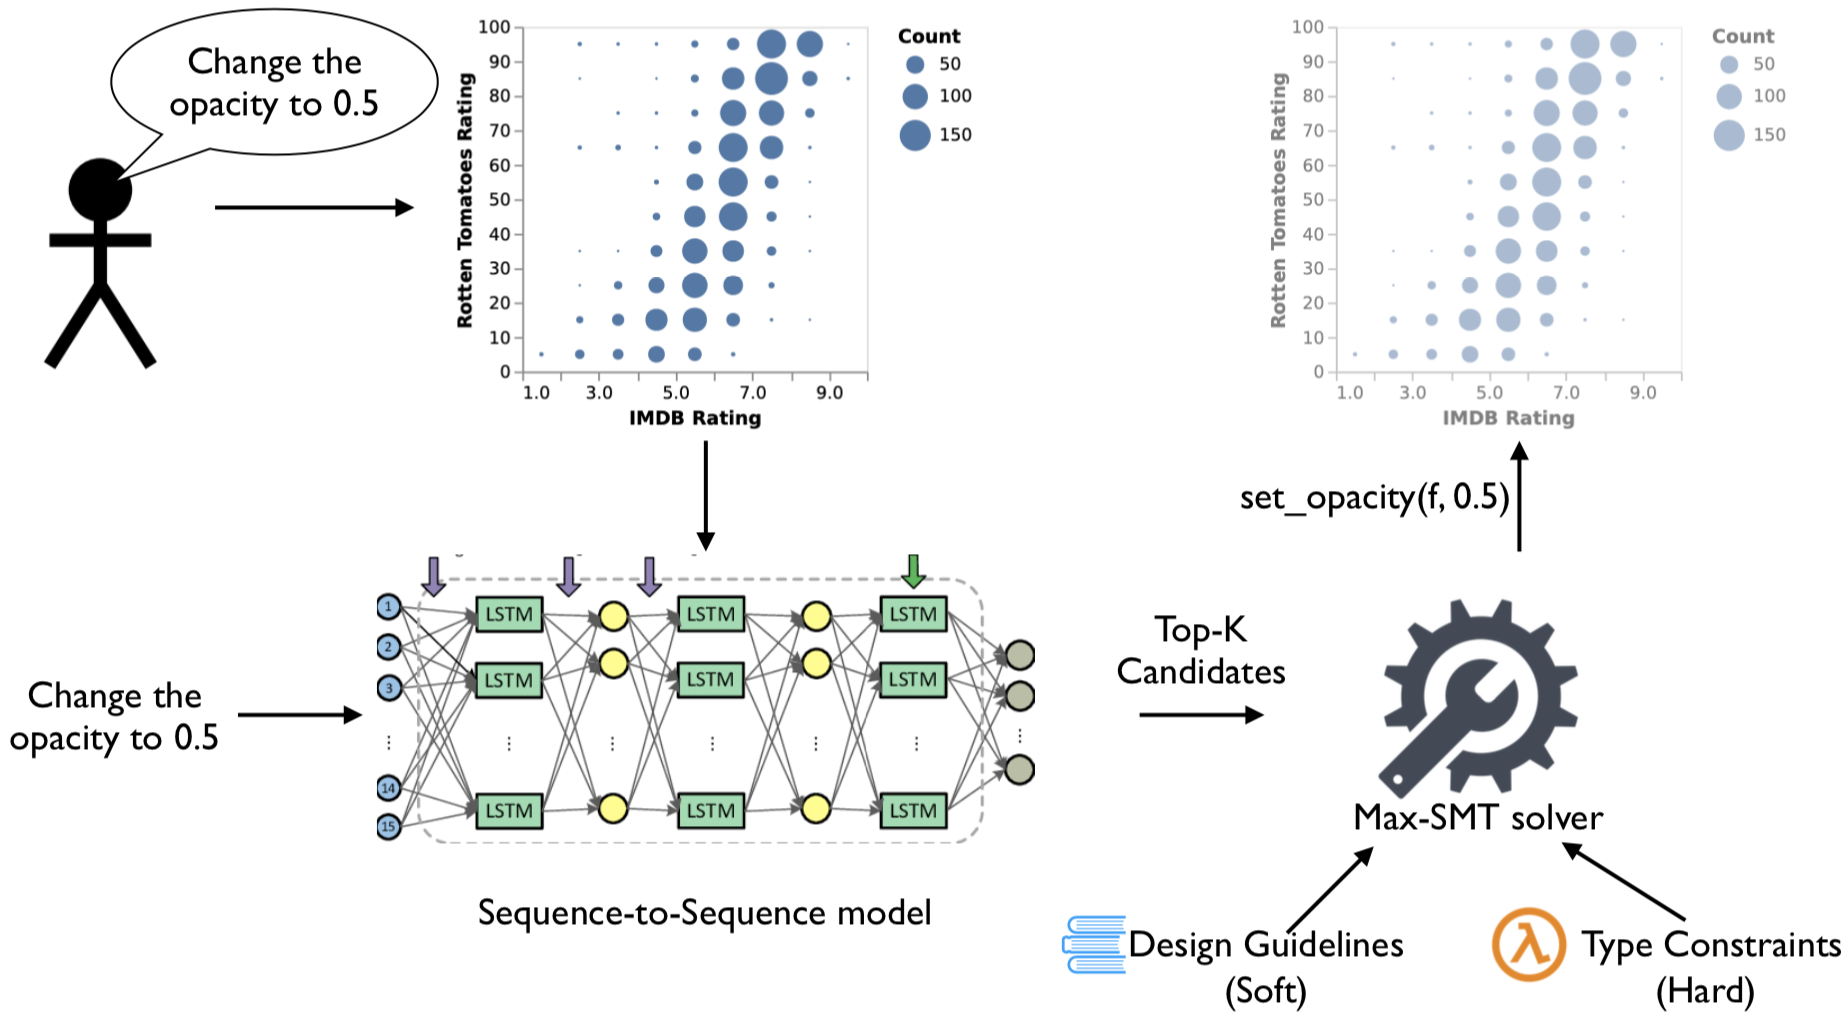
\includegraphics[height=22em,width=44em]{images/viz-overview.png}
}
%%%%%%%%%%%%%%%%%%%%%%%%%%%%%%%%%%%%%%%%%%%%%%%%%%%%%%%%%%%%%%%%%%%%%%%%%%%%%%
  \headerbox{References}{name=references,column=1,above=bottom}{
%%%%%%%%%%%%%%%%%%%%%%%%%%%%%%%%%%%%%%%%%%%%%%%%%%%%%%%%%%%%%%%%%%%%%%%%%%%%%%
    \smaller
    \bibliographystyle{ieee}
    \renewcommand{\section}[2]{\vskip 0.05em}
      \begin{thebibliography}{1}\itemsep=-0.01em
      \setlength{\baselineskip}{0.4em}
      \bibitem{amberg11:graphtrack}
        Yutong Shao and Ndapa Nakashole. 
        \newblock 
        CHARTDIALOGS: Plotting from Natural Language Instructions
        \newblock In {\em ACL,2020}
      \bibitem{awf:tracking}
        Chenglong Wang, Yu Feng, Ras Bodik, Alvin Cheung, Isil Dillig.
        \newblock 
        Visualization by Example.
        \newblock In {\em POPL 2020}
      \end{thebibliography}
   \vspace{0.3em}
  }
%%%%%%%%%%%%%%%%%%%%%%%%%%%%%%%%%%%%%%%%%%%%%%%%%%%%%%%%%%%%%%%%%%%%%%%%%%%%%%
  \headerbox{Future Work}{name=future,column=0,below=problem}{
%%%%%%%%%%%%%%%%%%%%%%%%%%%%%%%%%%%%%%%%%%%%%%%%%%%%%%%%%%%%%%%%%%%%%%%%%%%%%%
  \begin{multicols}{2}
We plan to continue our current work and integrate it into RStudio IDE to reduce the workload 
of daily program task; We also plan to train a model for large corpus of visualizations to generate more \emph{natural} visualizations.
Finally, currently our techniques only support Matplotlib in Python and we plan to extend our framework to support other languages like R and Java.

  \end{multicols}
   \vspace{0.3em}
  }
%%%%%%%%%%%%%%%%%%%%%%%%%%%%%%%%%%%%%%%%%%%%%%%%%%%%%%%%%%%%%%%%%%%%%%%%%%%%%%
  \headerbox{Acknowledgments}{name=ack,column=0,above=bottom,below=future}{
%%%%%%%%%%%%%%%%%%%%%%%%%%%%%%%%%%%%%%%%%%%%%%%%%%%%%%%%%%%%%%%%%%%%%%%%%%%%%%
We thank Yanju Chen in the PLSE lab for his unconditional support and guidance.
   \vspace{0.3em}
  }
%%%%%%%%%%%%%%%%%%%%%%%%%%%%%%%%%%%%%%%%%%%%%%%%%%%%%%%%%%%%%%%%%%%%%%%%%%%%%%
\headerbox{NEURAL ARCHITECTURE}{name=speed,column=2,span=2,row=0,below=results}{
  %%%%%%%%%%%%%%%%%%%%%%%%%%%%%%%%%%%%%%%%%%%%%%%%%%%%%%%%%%%%%%%%%%%%%%%%%%%%%%
  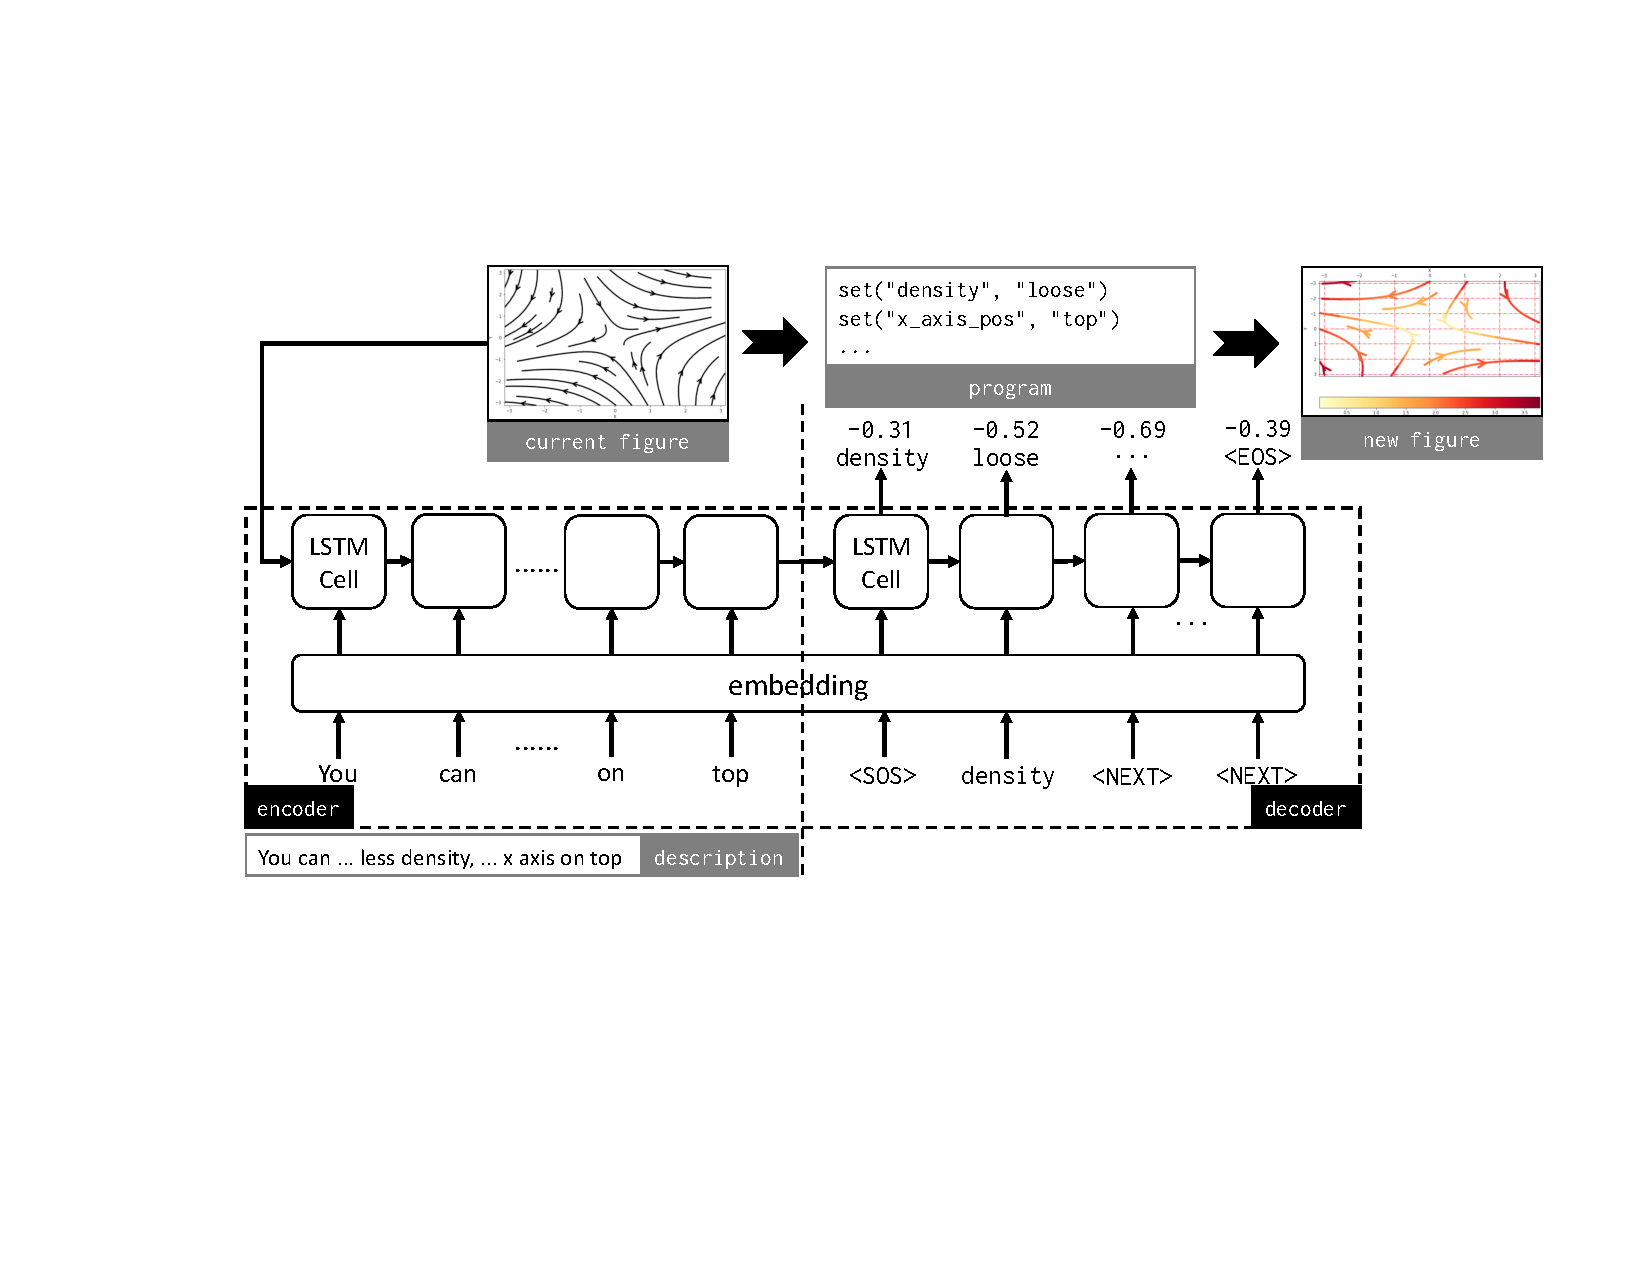
\includegraphics[height=22em,width=44em]{images/bsi_res.pdf}
   Given a \emph{question-solution} pair $(D, S)$, where a \emph{question} is a user description composed by word tokens $d$:
$D=(d_1, d_2, \ldots, d_n)$,
and a \emph{solution} is a symbolic program composed by a sequence of functions
$s_i$:
$S=(s_1, s_2, \ldots, s_m),$
the \emph{seq2seq} model is used to estimate the probability of $P(S|D)$, which is then given by:
$P(S|D)=P(s_1, s_2, \ldots, s_m|d_1, d_2, \ldots, d_n)=\prod_{t=1}^{m}P(s_t|v, s_1, s_2, \ldots, s_{t-1})$.
}
%%%%%%%%%%%%%%%%%%%%%%%%%%%%%%%%%%%%%%%%%%%%%%%%%%%%%%%%%%%%%%%%%%%%%%%%%%%%%%
%  \headerbox{Challenges}{name=method,column=0,below=problem,bottomaligned=speed}{
%%%%%%%%%%%%%%%%%%%%%%%%%%%%%%%%%%%%%%%%%%%%%%%%%%%%%%%%%%%%%%%%%%%%%%%%%%%%%%
%   \begin{itemize}\compresslist
%   \item {\bf \emph{Context abstraction:}} Identify a good abstraction of program context to drive database queries for discovering relevant components
%   \item {\bf \emph{Interface alignment:}} Once we identify relevant component, figure out correspondence between this component's interface and existing context elements
%   \item {\bf \emph{Adaptor code synthesis:}} We need to synthesize adaptor code to integrate component into program context 
%   \end{itemize}
%   \vspace{0.3em}
%  }
%%%%%%%%%%%%%%%%%%%%%%%%%%%%%%%%%%%%%%%%%%%%%%%%%%%%%%%%%%%%%%%%%%%%%%%%%%%%%%
  \headerbox{Our Solution}{name=solution,column=1,below=contribution,above=references}{
   \noindent{\centering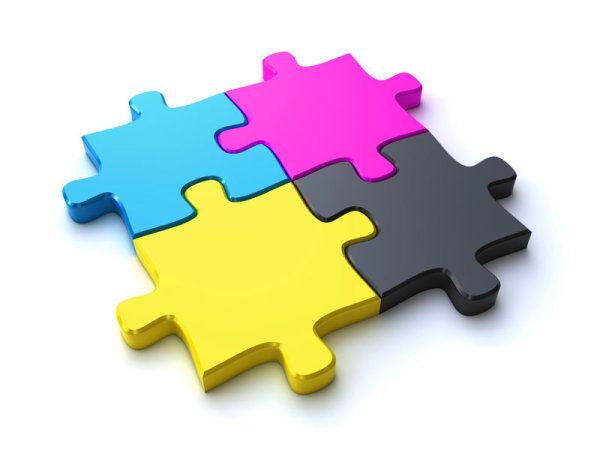
\includegraphics[width=0.45\linewidth]{images/pintu.jpg}\\}
 We combine the advantages of statistical and SMT-based techniques:
   \begin{enumerate}\itemsep=0.1cm
   \item Use LSTM to turn a natural language description into a set of candidate programs
   \item Use type-directed constraints to encode \emph{valid transformations}
   \item Use visualization design guidelines to encode \emph{recommended transformations}
   \item Formulate data visualization synthesis as a \emph{MAX-SMT} problem (i.e., find maximum cost matching that satisfies a set of integrity constraints)
   \end{enumerate}
 
  }

\end{poster}

\end{document}
